\documentclass{article}
\usepackage{graphicx} % new way of doing eps files
\usepackage{listings} % nice code layout
\usepackage[usenames]{color} % color
\definecolor{listinggray}{gray}{0.9}
\definecolor{graphgray}{gray}{0.7}
\definecolor{ans}{rgb}{1,0,0}
\definecolor{blue}{rgb}{0,0,1}
% \Verilog{title}{label}{file}
\newcommand{\Verilog}[3]{
  \lstset{language=Verilog}
  \lstset{backgroundcolor=\color{listinggray},rulecolor=\color{blue}}
  \lstset{linewidth=\textwidth}
  \lstset{commentstyle=\textit, stringstyle=\upshape,showspaces=false}
  \lstset{frame=tb}
  \lstinputlisting[caption={#1},label={#2}]{#3}
}


\author{Josh Young}
\title{Lab 8}

\begin{document}
\maketitle

\section{Introduction}
In Lab 6, the user is required to complete the ALU and ALU control. These 2 devices are an intergral part of the execute stage, where the ALU does the assigned arithmetic command based off of what the ALU control sends for an ALUOp code. Once the two modules where complete, testbenches were created to test and observe the outputs of the ALU and ALU control in order to ensure the proper behavior of each module. Vivado was used to create the test bench as well as run the simulation for the ALU and ALU control.

\section{Interface}
The ALU has two input, two outputs, and a control wire. The first input comes from a buffer that was fed with the register at RS from the regfile. The other input for the ALU comes from a mux that chooses between the Register at RT and the sign extender. One of the outputs for the ALU is the zero flag, which returns a 1 if the arithmetic result was zero. The other output is simply the result of the arithmetic operation. The control wire for the ALU comes from the ALU control, and tells the ALU what arithmetic operation to perform.
The ALU control has 1 input and two control wires. The ALU control gets its input from the first 6 bits of the sign extender. The control wires for the ALU control give the ALU operation and tell the ALU what to do.


\section{Design}
The ALU and ALU control are used as part of the execute stage, and are used in conjunction to provide the next program count as well as other arithmetic operations. These two modules define most of the execute stage since the only other components required for the design are a mux and a buffer.

\section{Implementation}
The code used for creating the ALU can be seen in Listing~\ref{code:ALU} on page~\pageref{code:ALU}. The code used for creating the ALU control can be seen in Listing~\ref{code:ALUcontrol} on page~\pageref{code:ALUcontrol}.

\Verilog{Verilog code for implementing the ALU.}{code:ALU}{../code/3_execute/ALU.v}
\Verilog{Verilog code for implementing the ALU control.}{code:ALUcontrol}{../code/2_decode/ALU_control.v}

\section{Test Bench Design}
The lab had the user create a test bench for both the ALU and ALU control. For the ALU, this was done by initializing to values, and then changing the ALU operation and view the result and zero flag. For the ALU control module, this was done by changing the op code and function code and observing the module's behavior.  
The verilog code for the ALU test bench can be viewed in Listing~\ref{code:ALUtest} on page~\pageref{code:ALUtest}. The verilog code for the ALU control test bench can be viewed in Listing~\ref{code:ALUctest} on page~\pageref{code:ALUctest}. 

\Verilog{Verilog code for testing the ALU.}{code:ALUtest}{../code/3_execute/ALU_test.v}
\Verilog{Verilog code for testing the ALU.}{code:ALUctest}{../code/3_execute/ALU_control_test.v}

\section{Simulation}
By viewing the timing diagrams for both the ALU and ALU control, one can deduce that they both behaved correctly. The timing diagram for the ALU can be viewed in Figure~\ref{fig:test}. The timing diagram for the ALU control can be viewed in Figure~\ref{fig:test2}. 
\section{Conclusions}
The goal for lab 8 was to complete the ALU and ALU control as well as test the two modules in order to ensure that both of them showed no bugs when observing the timing diagram. The simulation shows that the ALU and ALU control acted as it should have. 
\begin{figure}
	\begin{center}
		\caption{Timing diagram for the ALU test.}\label{fig:test}
		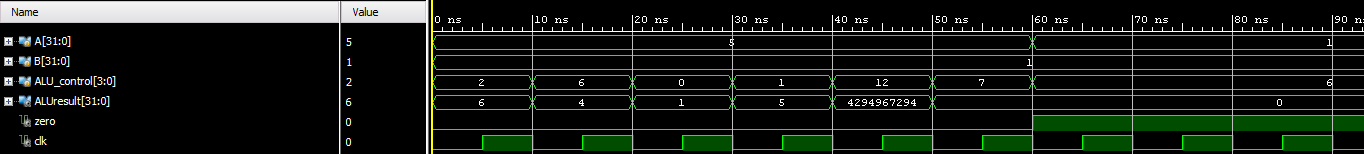
\includegraphics[width=0.9\textwidth]{../images/ALU_test.png}
	\end{center}
\end{figure}

\begin{figure}
	\begin{center}
		\caption{Timing diagram for the ALU control test.}\label{fig:test2}
		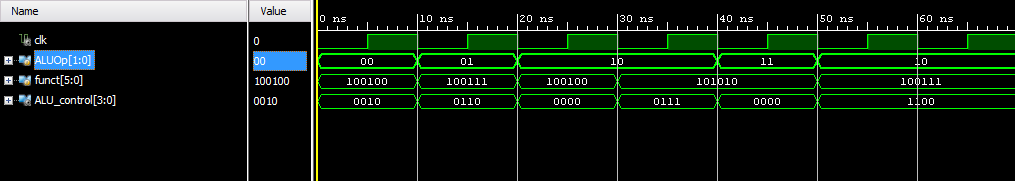
\includegraphics[width=0.9\textwidth]{../images/ALU_control_test.png}
	\end{center}
\end{figure}

\end{document} 